\documentclass[tikz,border=5pt]{standalone}
\usepackage[UTF8]{ctex}
\usepackage{amsmath,amssymb}
\usetikzlibrary{arrows.meta,calc,decorations.pathmorphing}
\tikzset{>=Stealth,line cap=round,line join=round,
motion/.style={blue!70!black,thick,->},
current/.style={red!70!black,thick,->},
aux/.style={black!40,dashed,thin},
dimension/.style={black!65,<->,thin}}
\newcommand{\fieldcross}[2]{
\draw[black!55] (#1,#2)circle(.10);
\draw[black!55] (#1-.065,#2-.065)--(#1+.065,#2+.065);
\draw[black!55] (#1-.065,#2+.065)--(#1+.065,#2-.065);
}
\newcommand{\railplane}{
\fill[black!3](0,0)--(3.2,0)--(4.2,1.2)--(1,1.2)--cycle;
\draw[thick](0,0)--(3.2,0);
\draw[thick](1,1.2)--(4.2,1.2);
\draw[very thick](1.2,0)--(2.2,1.2);
\draw[->](-.65,.15)--(.30,.15)node[below]{$x$};
\draw[->](-.65,.15)--(-.13,.774)node[above left]{$y$};
\draw[->](-.65,.15)--(-.65,1.5)node[above]{$z$};
\draw[current](3.6,2.45)--(3.6,1.48)node[midway,right]{$\boldsymbol B$};
}
\newcommand{\modeframe}{
\draw[thick](-.65,0)--(4,0);
\draw[thick](-.65,2)--(4,2);
\draw[thick](-.65,0)--(-.65,.88);
\draw[thick](-.99,.88)--(-.31,.88);
\draw[thick](-.99,1.12)--(-.31,1.12);
\draw[thick](-.65,1.12)--(-.65,2);
\node[left]at(-1.02,1){$C$};
\draw[very thick](1,0)--(1,2);
\draw[very thick](3,0)--(3,2);
\node[above]at(1,2){杆1};
\node[above]at(3,2){杆2};
}
\begin{document}
% 1: genuine plan view. Rods touch both continuous rails, capacitor bridges rails.
\begin{tikzpicture}[font=\small]
\draw[thick](0,0)--(6.2,0);
\draw[thick](0,3)--(6.2,3);
\draw[thick](0,0)--(0,1.34);
\draw[thick](-.45,1.34)--(.45,1.34);
\draw[thick](-.45,1.66)--(.45,1.66);
\draw[thick](0,1.66)--(0,3);
\node[left]at(-.48,1.5){$C$};
\node[right]at(.54,1.75){$+Q_0$};
\node[right]at(.54,1.25){$-Q_0$};
\foreach \xx in{2.7,5}{
\draw[very thick](\xx,0)--(\xx,3);
\fill(\xx,0)circle(1.5pt);
\fill(\xx,3)circle(1.5pt);
}
\node[above]at(2.7,3.15){杆1：$m,L$};
\node[above]at(5,3.15){杆2：$m,L$};
\fieldcross{1.35}{.70}\fieldcross{1.35}{2.30}
\fieldcross{3.80}{.70}\fieldcross{3.80}{2.30}
\node at(3.80,1.5){$B$};
\draw[black!40,thin](6.2,0)--(6.95,0);
\draw[black!40,thin](6.2,3)--(6.95,3);
\draw[dimension](6.75,0)--(6.75,3)node[midway,right]{$l$};
\draw[motion](5,-.55)--(3.95,-.55)node[midway,below]{$v_0$};
\draw[->](4.5,-1.30)--(6.2,-1.30)node[right]{$x$};
\node[below]at(5.35,-1.30){向右为正};
\end{tikzpicture}
% 2: actual 3D projection; x along rails, y across rails, z normal upward.
\begin{tikzpicture}[font=\small]
\begin{scope}
\railplane
\draw[motion](1.7,.6)--(2.85,.6);
\node[below,blue!70!black]at(2.65,.49){$v_j>0$};
\draw[motion](1.15,.18)--(1.85,1.02);
\node[above left,blue!70!black]at(1.55,.76){$\boldsymbol v_j\times\boldsymbol B$};
\node at(1.8,-.63){动生电动势指向上导轨};
\end{scope}
\begin{scope}[xshift=6.4cm]
\railplane
\draw[current](1.34,.168)--(2.02,.984);
\node[right,red!70!black]at(2.05,.99){$I_j>0$};
\draw[motion](1.7,.6)--(.50,.6);
\node[below,blue!70!black]at(1.10,.51){$\boldsymbol F_j$};
\node at(1.8,-.63){安培力沿导轨向左};
\end{scope}
\end{tikzpicture}
% 3: two parallel moving-inductive branches; upper polarity of emf is positive
% only for positive v_j; all arrows designate reference directions.
\begin{tikzpicture}[font=\small]
\draw[thick](0,0)--(6.6,0);
\draw[thick](0,4)--(6.6,4);
\draw[thick](0,0)--(0,1.87);
\draw[thick](-.42,1.87)--(.42,1.87);
\draw[thick](-.42,2.13)--(.42,2.13);
\draw[thick](0,2.13)--(0,4);
\node[left]at(-.45,2){$C$};
\node[right]at(.50,2.20){$q$};
\node[right]at(.50,1.80){$-q$};
\draw[<->,black!60](-1.15,.05)--(-1.15,3.95);
\node[left]at(-1.15,2){$U=q/C$};
\foreach \xx/\jj in{3/1,6/2}{
\draw[thick](\xx,0)--(\xx,.65);
\draw[thick](\xx,1.35)--(\xx,2.48);
\draw[thick,decorate,decoration={coil,aspect=.45,amplitude=2.5pt,segment length=5pt}](\xx,2.48)--(\xx,3.32);
\draw[thick](\xx,3.32)--(\xx,4);
\draw[thick](\xx,1)circle(.35);
\node at(\xx,1.17){$+$};
\node at(\xx,.83){$-$};
\node[right]at(\xx+.48,1){$\varepsilon_{\jj}=\kappa v_{\jj}$};
\node[right]at(\xx+.36,2.90){$L$};
\draw[current](\xx-.5,2.20)--(\xx-.5,3.15);
\node[left,red!70!black]at(\xx-.50,2.68){$I_{\jj}$};
\fill(\xx,0)circle(1.5pt);
\fill(\xx,4)circle(1.5pt);
}
\node[above]at(4.5,4.12){上导轨};
\node[below]at(4.5,-.12){下导轨};
\end{tikzpicture}
% 4: representative positions, not a time plot. Physical coordinates X vs
% displacements x are separated; C0 midpoint 3.4, C(t) midpoint 3.15.
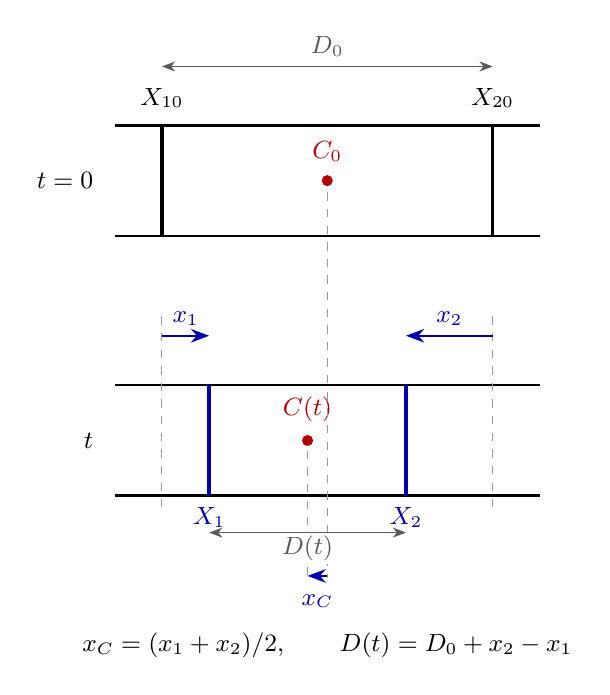
\begin{tikzpicture}[font=\small]
\draw[thick](.7,3.30)--(6.1,3.30);
\draw[thick](.7,4.70)--(6.1,4.70);
\draw[very thick](1.3,3.30)--(1.3,4.70);
\draw[very thick](5.5,3.30)--(5.5,4.70);
\node[left]at(.55,4){$t=0$};
\node[above]at(1.3,4.80){$X_{10}$};
\node[above]at(5.5,4.80){$X_{20}$};
\fill[red!70!black](3.4,4)circle(2pt);
\node[above,red!70!black]at(3.4,4.12){$C_0$};
\draw[dimension](1.3,5.45)--(5.5,5.45)node[midway,above]{$D_0$};
\draw[thick](.7,0)--(6.1,0);
\draw[thick](.7,1.4)--(6.1,1.4);
\draw[aux](1.3,-.15)--(1.3,2.30);
\draw[aux](5.5,-.15)--(5.5,2.30);
\draw[very thick,blue!70!black](1.9,0)--(1.9,1.4);
\draw[very thick,blue!70!black](4.4,0)--(4.4,1.4);
\node[left]at(.55,.70){$t$};
\node[below,blue!70!black]at(1.9,-.03){$X_1$};
\node[below,blue!70!black]at(4.4,-.03){$X_2$};
\draw[motion](1.3,2.03)--(1.9,2.03)node[midway,above]{$x_1$};
\draw[motion](5.5,2.03)--(4.4,2.03)node[midway,above]{$x_2$};
\fill[red!70!black](3.15,.70)circle(2pt);
\node[above,red!70!black]at(3.15,.82){$C(t)$};
\draw[aux](3.4,3.85)--(3.4,-1.05);
\draw[aux](3.15,.57)--(3.15,-1.05);
\draw[dimension](1.9,-.47)--(4.4,-.47)node[midway,below,fill=white,inner sep=1pt]{$D(t)$};
\draw[motion](3.4,-1.02)--(3.15,-1.02);
\node[below,blue!70!black]at(3.275,-1.13){$x_C$};
\node at(3.4,-1.90){$x_C=(x_1+x_2)/2,\qquad D(t)=D_0+x_2-x_1$};
\end{tikzpicture}
% 5: modal components. Arrows are positive reference component directions,
% not a claim that all actual initial currents are positive.
\begin{tikzpicture}[font=\small]
\begin{scope}
\modeframe
\node at(1.5,2.95){同向分量：$\Omega$};
\draw[current](1,.35)--(1,1.65);
\draw[current](3,.35)--(3,1.65);
\node[left,red!70!black]at(.85,1){$i/2$};
\node[right,red!70!black]at(3.15,1){$i/2$};
\draw[motion](1,-.38)--(1.8,-.38)node[midway,below]{$u$};
\draw[motion](3,-.38)--(3.8,-.38)node[midway,below]{$u$};
\node at(1.5,-1.20){$v_1=v_2=u,\quad I_1+I_2=i$};
\end{scope}
\begin{scope}[xshift=6.4cm]
\modeframe
\node at(1.5,2.95){反向分量：$\omega_0$};
\draw[current](1,1.65)--(1,.35);
\draw[current](3,.35)--(3,1.65);
\node[left,red!70!black]at(.85,1){$J/2$};
\node[right,red!70!black]at(3.15,1){$J/2$};
\draw[motion](1,-.38)--(.20,-.38)node[midway,below]{$\delta/2$};
\draw[motion](3,-.38)--(3.8,-.38)node[midway,below]{$\delta/2$};
\node at(1.5,-1.20){$v_1=-\delta/2,\quad v_2=\delta/2$};
\node at(1.5,-1.77){$I_1=-J/2,\quad I_2=J/2$};
\end{scope}
\end{tikzpicture}
% 6: actual phase directions: common mode CW from +x; relative mode CCW
% from -x. Normalized orbit points use the same illustrative phase 55 degrees.
\begin{tikzpicture}[font=\small]
\begin{scope}
\draw[->](-1.9,0)--(2.0,0)node[right]{$q/Q_0$};
\draw[->](0,-1.8)--(0,1.8)node[above]{$\dot q/(\Omega Q_0)$};
\draw[thick,blue!70!black](0,0)circle(1.4);
\fill[red!70!black](1.4,0)circle(2pt);
\node[below right,red!70!black]at(1.4,-.13){初态};
\draw[aux](0,0)--(.803,-1.147);
\fill[blue!70!black](.803,-1.147)circle(2pt);
\draw[motion](1.379,-.243)arc[start angle=-10,end angle=-40,radius=1.4];
\draw[thin,->](.43,0)arc[start angle=0,end angle=-55,radius=.43];
\node at(.69,-.40){$\Omega t$};
\node at(0,2.56){电荷同向模};
\node at(0,-2.20){$(\cos\Omega t,\,-\sin\Omega t)$};
\end{scope}
\begin{scope}[xshift=6.7cm]
\draw[->](-1.9,0)--(2.0,0)node[right]{$\delta/v_0$};
\draw[->](0,-1.8)--(0,1.8)node[above]{$J/(Q_0\omega_0)$};
\draw[thick,blue!70!black](0,0)circle(1.4);
\fill[red!70!black](-1.4,0)circle(2pt);
\node[below left,red!70!black]at(-1.4,-.13){初态};
\draw[aux](0,0)--(-.803,-1.147);
\fill[blue!70!black](-.803,-1.147)circle(2pt);
\draw[motion](-1.379,-.243)arc[start angle=190,end angle=220,radius=1.4];
\draw[thin,->](-.43,0)arc[start angle=180,end angle=235,radius=.43];
\node at(-.69,-.40){$\omega_0t$};
\node at(0,2.56){相对运动模};
\node at(0,-2.20){$(-\cos\omega_0t,\,-\sin\omega_0t)$};
\end{scope}
\end{tikzpicture}
\end{document}
